\documentclass{standalone}
%\usetikzlibrary{...}
\usepackage{tikz}
\begin{document}
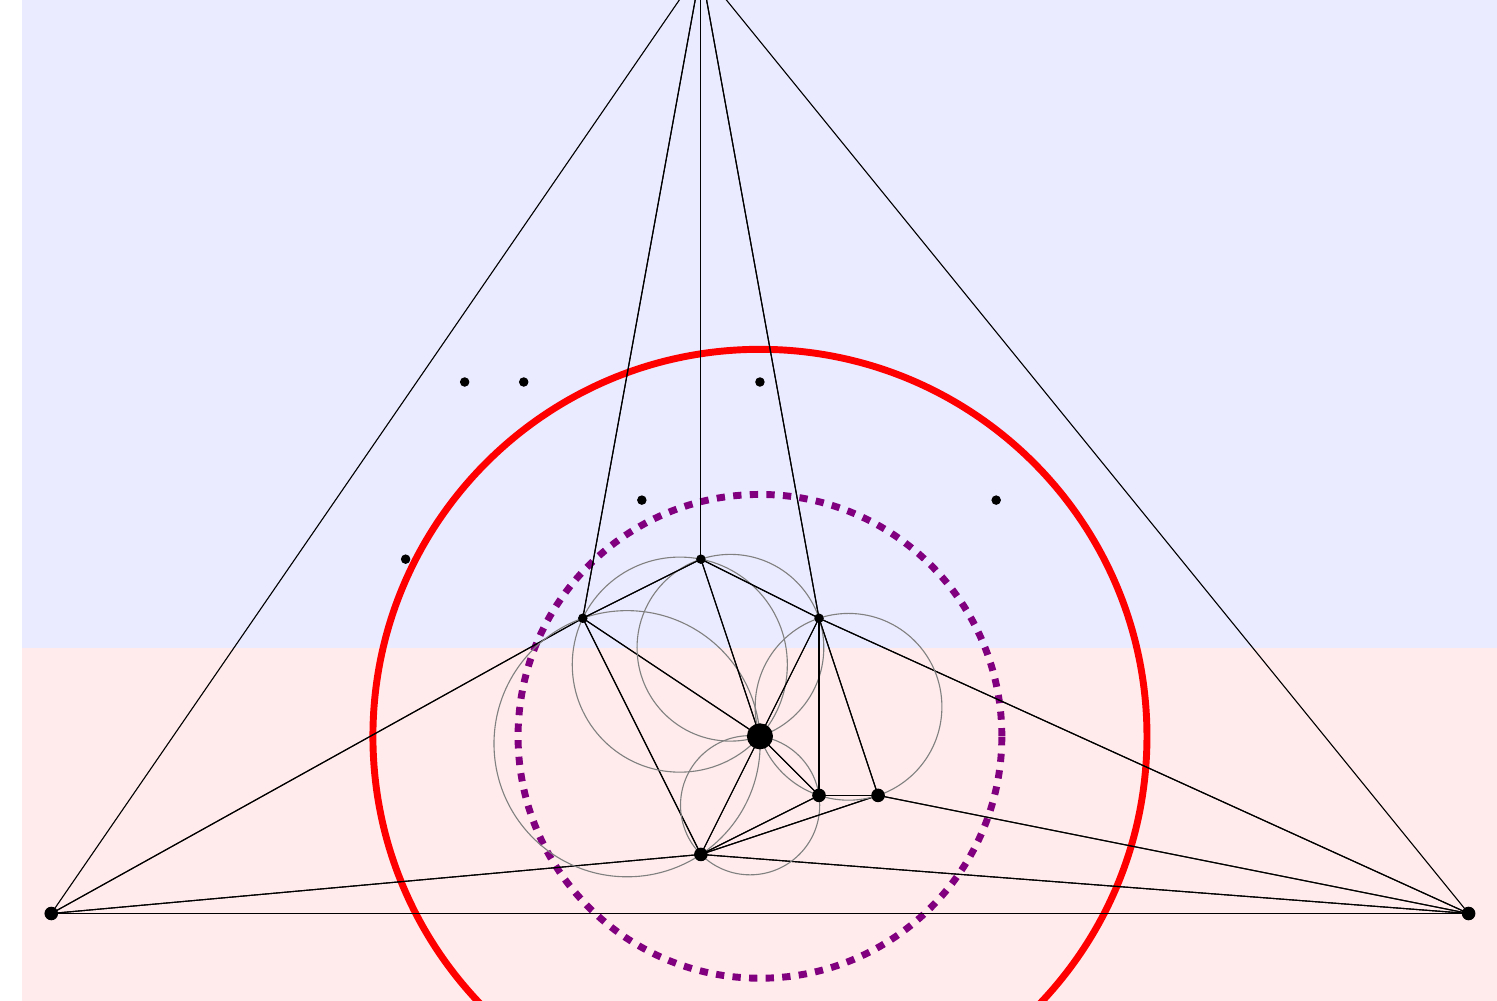
\begin{tikzpicture}[scale=1.5]
\path[use as bounding box] (-6.2, -2) rectangle (6, 6);

\tikzstyle{main_point} = [radius=3pt, blue];
\tikzstyle{present_point} = [radius=1.5pt, red!30!gray];
\tikzstyle{hidden_point} = [radius=1pt, blue!30!gray];
\tikzstyle{circ} = [gray, line width=0.4];
\tikzstyle{test_circle} = [red, line width=2.5];
\tikzstyle{old_test_circle} = [violet, line width=2.5];
\fill [red!8!white] (-6.25, -3.5) rectangle (6.25, 0.75);
\fill [blue!8!white] (-6.25, 0.75) rectangle (6.25, 6.75);
\draw[old_test_circle, dashed] (0, 0) circle (2.048);
\draw[test_circle] (0, 0) circle (3.2768);
\draw (-1.5, 1.0) -- (-0.5, 6.5);
\draw (-0.5, 6.5) -- (-6.0, -1.5);
\draw (-6.0, -1.5) -- (-1.5, 1.0);
\draw (6.0, -1.5) -- (-0.5, -1.0);
\draw (-0.5, -1.0) -- (-6.0, -1.5);
\draw (-6.0, -1.5) -- (6.0, -1.5);
\draw (-0.5, -1.0) -- (-1.5, 1.0);
\draw (-1.5, 1.0) -- (-6.0, -1.5);
\draw (-6.0, -1.5) -- (-0.5, -1.0);
\draw (-1.5, 1.0) -- (-0.5, -1.0);
\draw (-0.5, -1.0) -- (0.0, 0.0);
\draw (0.0, 0.0) -- (-1.5, 1.0);
\draw[circ] (-1.125, -0.0625) circle(1.1267347735824966);
\draw (-0.5, 6.5) -- (0.5, 1.0);
\draw (0.5, 1.0) -- (6.0, -1.5);
\draw (6.0, -1.5) -- (-0.5, 6.5);
\draw (1.0, -0.5) -- (-0.5, -1.0);
\draw (-0.5, -1.0) -- (6.0, -1.5);
\draw (6.0, -1.5) -- (1.0, -0.5);
\draw (0.5, 1.0) -- (1.0, -0.5);
\draw (1.0, -0.5) -- (6.0, -1.5);
\draw (6.0, -1.5) -- (0.5, 1.0);
\draw (-0.5, 1.5) -- (-1.5, 1.0);
\draw (-1.5, 1.0) -- (0.0, 0.0);
\draw (0.0, 0.0) -- (-0.5, 1.5);
\draw[circ] (-0.6785714285714286, 0.6071428571428572) circle(0.9105391988558543);
\draw (0.5, 1.0) -- (-0.5, 1.5);
\draw (-0.5, 1.5) -- (0.0, 0.0);
\draw (0.0, 0.0) -- (0.5, 1.0);
\draw[circ] (-0.25, 0.75) circle(0.7905694150420949);
\draw (-1.5, 1.0) -- (-0.5, 1.5);
\draw (-0.5, 1.5) -- (-0.5, 6.5);
\draw (-0.5, 6.5) -- (-1.5, 1.0);
\draw (-0.5, 1.5) -- (0.5, 1.0);
\draw (0.5, 1.0) -- (-0.5, 6.5);
\draw (-0.5, 6.5) -- (-0.5, 1.5);
\draw (-0.5, -1.0) -- (0.5, -0.5);
\draw (0.5, -0.5) -- (0.0, 0.0);
\draw (0.0, 0.0) -- (-0.5, -1.0);
\draw[circ] (-0.08333333333333331, -0.5833333333333334) circle(0.5892556509887896);
\draw (1.0, -0.5) -- (0.5, -0.5);
\draw (0.5, -0.5) -- (-0.5, -1.0);
\draw (-0.5, -1.0) -- (1.0, -0.5);
\draw (0.5, -0.5) -- (1.0, -0.5);
\draw (1.0, -0.5) -- (0.5, 1.0);
\draw (0.5, 1.0) -- (0.5, -0.5);
\draw (0.5, -0.5) -- (0.5, 1.0);
\draw (0.5, 1.0) -- (0.0, 0.0);
\draw (0.0, 0.0) -- (0.5, -0.5);
\draw[circ] (0.75, 0.25) circle(0.7905694150420949);
\filldraw (0.0, 0.0) circle[main_point];
\filldraw (1.0, -0.5) circle[present_point];
\filldraw (0.5, -0.5) circle[present_point];
\filldraw (-0.5, -1.0) circle[present_point];
\filldraw (-0.5, 6.5) circle[present_point];
\filldraw (-6.0, -1.5) circle[present_point];
\filldraw (6.0, -1.5) circle[present_point];
\filldraw (-1.5, 1.0) circle[hidden_point];
\filldraw (-0.5, 1.5) circle[hidden_point];
\filldraw (0.5, 1.0) circle[hidden_point];
\filldraw (2.0, 2.0) circle[hidden_point];
\filldraw (-2.0, 3.0) circle[hidden_point];
\filldraw (-2.5, 3.0) circle[hidden_point];
\filldraw (-3.0, 1.5) circle[hidden_point];
\filldraw (-1.0, 2.0) circle[hidden_point];
\filldraw (0.0, 3.0) circle[hidden_point];

\end{tikzpicture}
\end{document}
